\section{Conclusion and Work Plan}
\label{sec:conclusion}
The pilot work just shown is exciting and compelling, and demonstrates the value of our proposed work. First,
 we are able to verify the most comprehensive model of discrimination and its impact on behavior and outcomes to date.
 As illustrated in ~\ref{fig:model}, we hypothesize that discrimination's impact on mental and physical health will  impact those stress-related behaviors (\ref{itm:rq-behavior}). Our study will not only help to test that hypothesis but also to quantify the size and direction and longitudinal impact of discrimination on each type of behavior, thus improving our theoretical model of discrimination's impact on people (\ref{itm:rq-behavior-size}, \ref{itm:rq-severity-impact}).
 
 In addition, ours is the first model at this level of detail to tie discrimination specifically to student outcomes such as GPA and retention. Our model will help to link short term behavior to long-term outcomes (\ref{itm:rq-short-long}, \ref{itm:rq-which-long}, \ref{itm:rq-which-long}) This makes it extremely valuable for helping with intervention design and policy setting on university campuses.
 For example, the buffering effect of social support have implications for intervention design. 

Lastly, our approach is the first to explore the relationship between specific micro-climates and the mediating factors that help to buffer people from the impact of discrimination (\ref{itm:mc-daily-discrimination}, \ref{itm:mc-internal-mediators}, \ref{itm:mc-external-mediators}). By studying the impact of micro-climates on outcomes we can provide support for intervention design and further enrich our theoretical model. 

Educational institutions are characterized by dominant attitudes and behaviors. Some disciplines are particularly vulnerable to gender, race, and nationality bias, including  engineering \cite{sevo2010bias}.  We believe that it is critically important to study these issues in the educational context, a sentiment recently argued in an NSF Dear Colleague Letter encouraging research in sexual harassment and other forms or harrassment in STEM contexts \footnote{\url{www.nsf.gov/pubs/2019/nsf19053/}}. The pervasiveness of discrimination experiences in our data was a surprise to our team, and addressing them is critical to creating a diverse and informed workforce. This can only be done by shedding light on these darker aspects of engineering education. 
As Bill and Melinda Gates said in their  recent Annual Letter \footnote{\url{https://www.gatesnotes.com/2019-Annual-Letter}}, data is sexist (and racist) and the biases inherent in the data we collect are necessary, indeed critical to address. This study is a first attempt to do so, and we hope to contribute to the development of this domain as an important topic of study for computational researchers.   

%A comprehensive change in the way that we study the college student experience. 
%Our research facilitates this thanks to new changes in the ease of capturing real-time student information. Our work is innovative because it allows us to study the student experience at scale, provides before-after data around events such as discrimination,
% quantifies impact, and allow us to design the most effective interventions and policies.
 
Our work plan is as follows: 


%\begin{table}[]
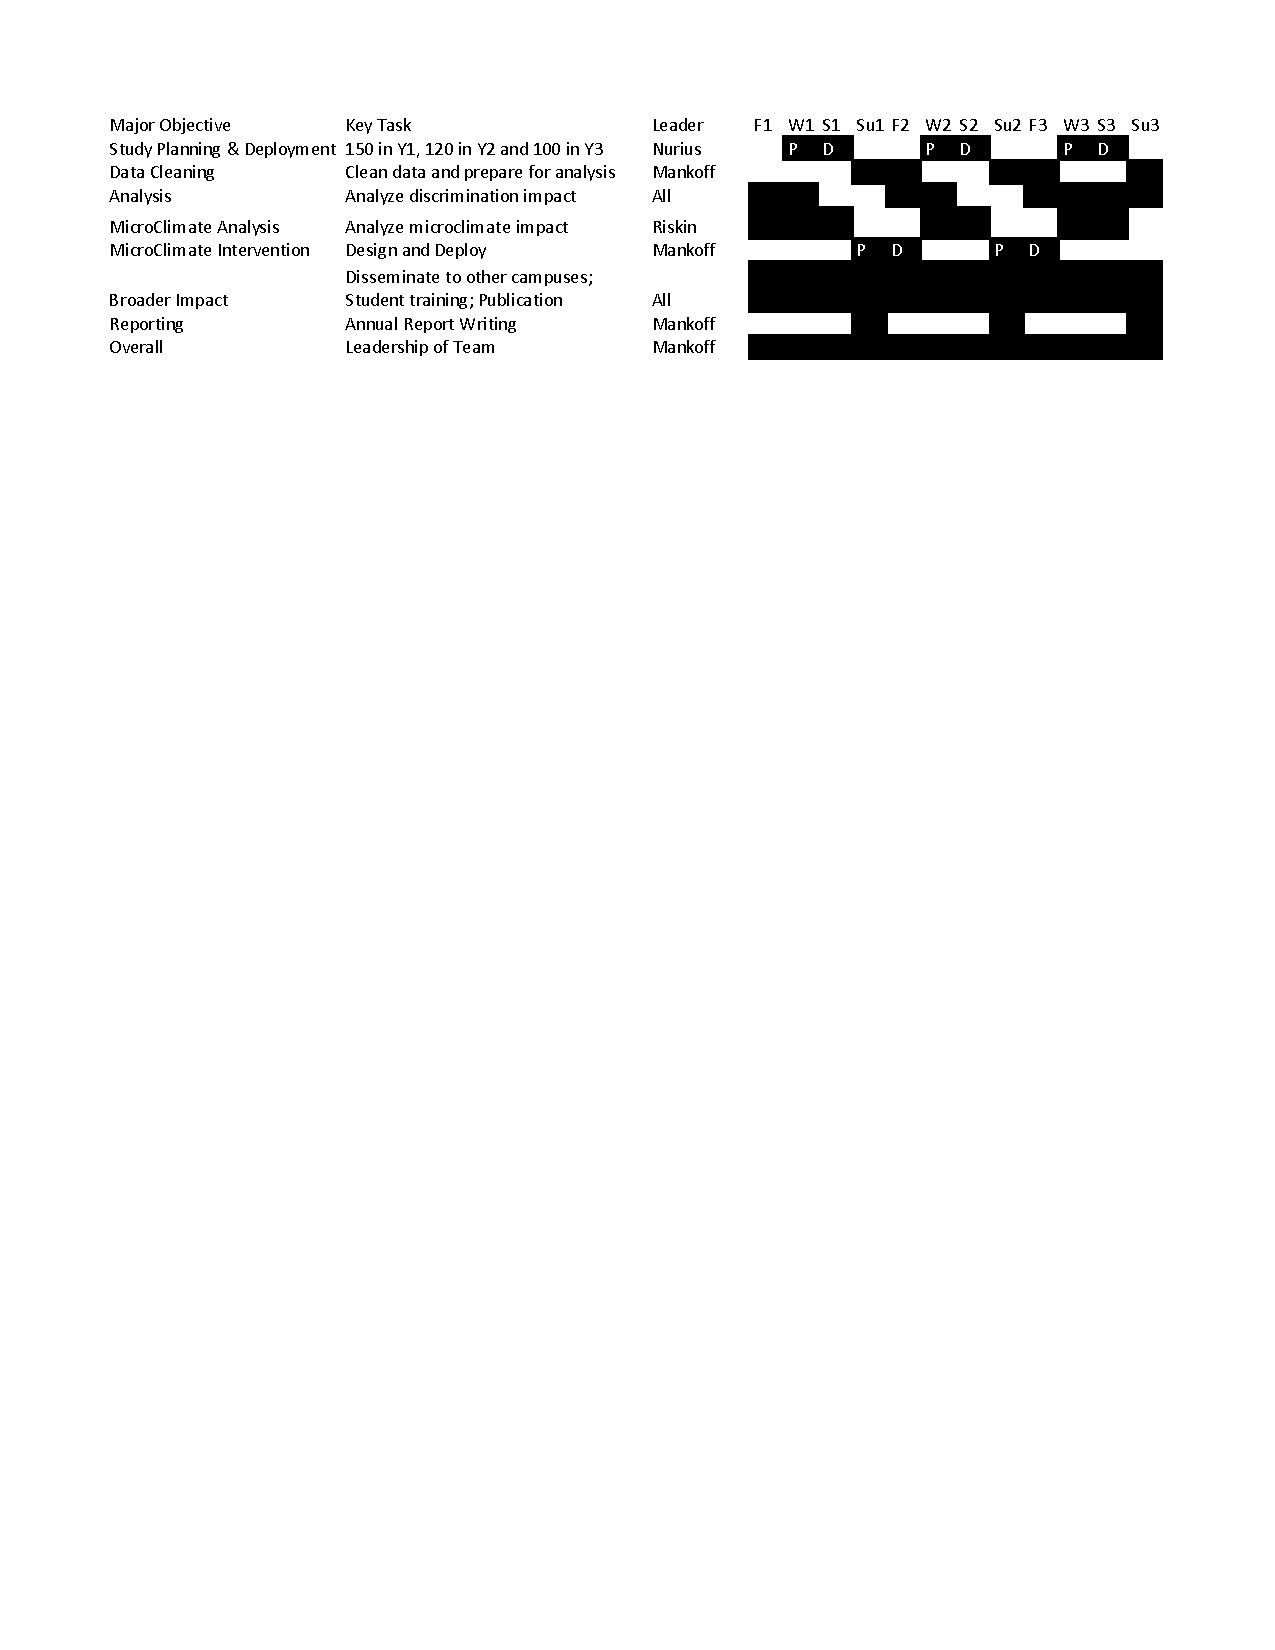
\includegraphics[width=\textwidth]{img/workplan.pdf}
% \small
% \resizebox{\textwidth}{
% \begin{tabular}{p{3cm}p{3cm}lllllllllllll}
% \textbf{Major Objective} &  \textbf{Key Task} & \textbf{Leader} &  F1 &  W1 & S1 & Su1 & F2 & W2 & S2 & Su2 & F3 & W3 & S3 & Su3 \\ \hline
% Study Planning \& Deployment & 150 in Y1, 120 in Y2 and 100 in Y3 & Nurius &  &  P &  D &  &  &  P & D &  &  & P & D &  \\
% Data Cleaning & Clean data and prepare for analysis & Mankoff &  &  &  & X & X &  & X & X &X &  &  & X \\
% Analysis & Analyze discrimination impact & All & X&X&  &  &X& X  &  &  & X & X & X & X\\
% Microclimate Analysis & Analyze microclimate impact & Riskin &X&X & X &  &  & X & X &  &  &X&X &  \\
% Microclimate Intervention & Design and Deploy & Mankoff &  &  &  & P & D &  &  &  P &  D &  &  &  \\
% Broader Impact & \begin{tabular}[c]{@{}l@{}}Disseminate to other campuses; \\ Student training; Publication\end{tabular} & All &  & X & X & X & X & X & X & X & X & X& X& X& X\\
% Reporting & Annual Report Writing & Mankoff &  &  &  & X &  &  &  & X &  &  &  & X \\
% Overall & Leadership of Team & Mankoff & X & X & X & X & X & X & X & X & X& X& X& X
% \end{tabular}%
% }
%\end{table}